\chapterimage{Laboratory}

\chapter{Constituents Properties and Analysis}\index{Constituents Properties and Analysis}


\section{Wastewater Constituents} \index{Wastewater Constituents}
		\subsection{Organics}\index{Organics}		
		\begin{itemize}
			\item The main reason for treating domestic wastewater is to remove the organic matter.  
			\item Organics are substances containing carbon, hydrogen and oxygen, and some of which may be combined with nitrogen, sulfur or phosphorous.
			\item About 50 percent of the solids present in wastewater are organic.  This fraction is generally of animal or vegetable life, dead animal matter, plant tissue or organisms, and also include synthetic organic compounds.
			\item The principal organic compounds present in domestic wastewater are proteins, carbohydrates and fats together with the products of their decomposition.
			\item Organics are subject to decay or decomposition through the activity of bacteria and other living organisms.  \hl{Since the organic fraction can be driven off at high temperatures, they are also called \textbf{volatile solids}}.\
			\item \emph{Organics in wastewater is typically quantified in terms of oxygen required to oxidize the carbon based material present} in wastewater using the following methods:\\
\subsubsection{Biochemical Oxygen Demand (BOD)}\index{Biochemical Oxygen Demand (BOD)}

			  %     \begin{enumerate}[i.]
			  %     	\definecolor{shadecolor}{RGB}{220,220,220}
					% %%%%%%%%%%%
					% % LEVEL 4 %
					% %%%%%%%%%%%
			  %     	\begin{snugshade*}
			  %     		\item \noindent\textsc{Biochemical Oxygen Demand (BOD)}%@@@@@@@@@@@@@@@@@@%
			  %     	\end{snugshade*}					
			      	\begin{itemize}
			      		\item Oxygen is required for the consumption of organic matter by aerobic bacteria
			      		\item BOD test measures the depletion of oxygen in a wastewater sample over a five day period
			      		\item BOD measures the organic content in terms of oxygen required for the microorganisms to consume the organic material present

			      		\item BOD is typically measured as BOD$_5$ which is the oxygen demand of the wastewater measured after 5 days of the initiation of the test.
			      		\item The test involves incubating a known dilution of wastewater in a 300 ml bottle for 5 days at 20\si{\degree}C.  The dissolved oxygen (DO) content at the start and end of the incubation period is used for calculating the BOD.
			      		\item For the test to be considered valid, the following criteria need to be met: 1) DO consumption during the test must be at least 2 mg/l, 2) DO remaining at the end of the test must be at least 1 mg/l, and 3) DO consumed in blank should be 0.2 mg/l or less
			      		      			
			      		\item BOD is a parameter to measure the strength of wastewater and the measurement of the wastewater treatment plant or treatment process influent and effluent BOD is standard practice to measure its performance.  Typical domestic wastewater BOD is about 200-250 mg/l.
			      		\item The oxygen consumed by the microorganisms during the BOD test is primarily for: 1) Oxidizing the carbonaceous material (cBOD – carbonaceous BOD), and 2) Oxidizing nitrogenous constituents such as ammonia (nBOD – nitrogenous BOD).
			      		\item Thus, BOD (Total) = cBOD + nBOD.  The cBOD and nBOD is measured by adding certain chemical inhibitors which will inhibit the bacteria responsible for consuming the nitrogenous matter, thus measuring only the cBOD as part of the BOD test.
			      		\item Since not all of the organics is metabolized in the 5 days of the regular BOD test, certain wastewater discharge permits require reporting of the ultimate BOD value (BOD$_U$)\\
			      	\end{itemize}

			    \subsubsection{Chemical Oxygen Demand (COD)}\index{Chemical Oxygen Demand (COD)}
			      	% \begin{snugshade*}
			      	% 	\item \noindent\textsc{Chemical Oxygen Demand (COD)}%@@@@@@@@@@@@@@@@@@%
			      	% \end{snugshade*}		  
			      	\begin{itemize}
			      		\item The COD test involves using chemical oxidizers to measure the oxygen demand of the wastewater.
			      		\item As the chemical oxidizers will oxidize other constituents present, including inorganic matter, the COD value of wastewater will be higher than the BOD.  
			      		\item The COD test can be conducted rather quickly than the 5 day BOD test, it is an effective method to quantify the wastewater strength and process efficiencies and allow operators to make timely process adjustments.
			      	\end{itemize}

			    \subsubsection{Total Organic Carbon (TOC)}
			      	% \begin{snugshade*}
			      	% 	\item \noindent\textsc{Total Organic Carbon (TOC):}\\%@@@@@@@@@@@@@@@@@@%
			      	% \end{snugshade*}
			      	The TOC method utilizes laboratory analytical instruments which directly measure the organic carbon content by quantifying the amount of carbon dioxide produced from the complete combustion of the organics present.
			      % \end{enumerate}
		\end{itemize}
		
		
		
			\hl{Note: BOD measures the amount of oxygen required by the microorganisms present to consume the organic material while COD measures the chemical oxidation required to oxidize all chemicals including organics present in wastewater.  BOD value of typical domestic sewage is about 200 - 250 mg/l while the COD value ranges from 300 - 450 mg/l.  Typical BOD:COD ratio ranges from 0.5-0.8.}\\


\subsection{Solids}\index{Solids}
% 		\pagebreak
% 				\begin{snugshade*}
% 			\item \noindent\textsc{Solids}
% 		\end{snugshade*}	
		Like BOD, wastewater solids is another critical parameter for establishing the wastewater strength and determining treatment process efficiencies. 
		\begin{itemize}
			\item The \texthl{solids can be classified as suspended or dissolved} based upon its ability to pass through a standardized filter paper.
			\item When the wastewater is filtered:
			      \begin{itemize}
			      	\item the residual solids remaining on the filter paper after drying in an oven at 103\si{\degree}C is the \hl{suspended solids} portion, and 
			      	\item the solids remaining after drying the filtrate are the \hl{dissolved solids}.
			      \end{itemize}
			\item Suspended solids include larger floating particles and consist of sand, grit, clay, fecal matter, paper, pieces of wood, particles of food and garbage, and similar materials.
			\item Suspended solids can be categorized based upon its settling characteristics as:
			      \begin{itemize}
			      	\item \hl{Settleable}
			      	\item \hl{Non-settleable}
			      	      \begin{itemize}
			      	      	\item \hl{Colloidial}-small, charged (typically negative) particles which do not settle easily.  Some of the colloidial particles are small enough to pass through the filter paper used for filtering the suspended solids
			      	      	\item \hl{Floatable}-example oil and grease and small plastics
			      	      \end{itemize}
			      \end{itemize}
			\item Dissolved solids in wastewater include organics.  However, the major elements of dissolved solids are inorganic ions such as Ca$^{+2}$, Mg$^{+2}$, Cl$^-$, SO$_4$ $^{-2}$ , HCO$_3$ $^-$, Fe$^{+2}$, PO$_4$ $^{-3}$, NO$_3$ $^-$.  These ions are part of the dissolved salts such as sodium chloride (NaCl), calcium bicarbonate (Ca(HCO$_3$)$_2$), magnesium phosphate (Mg$_3$PO$_4$) and others which are normally present in water and wastewater. 
			      \begin{itemize}
			      	\item Conductivity or electrical conductance (EC) measurement is typically conducted as the wastewater enters the plant as \hl{conductivity provides an indirect and simple measure of the amount of dissolved solids present.}  
			      	\item Conductivity or electrical conductance (EC) is a measure the amount of electrical current that can be conducted by a solution.  
			      	\item The conductance of electricity in a solution is due to the presence of dissolved inorganic ions 
			      	\item The higher the concentration of these ions, the higher is the conductivity. 
			      	\item \underline{Conductivity is measured in the units of mhos/cm or Siemens/cm.}  (Note:  mhos is the reverse of ohm which is a measure of resistance).
			      	\item Typical wastewater conductivities range from 50 to 1500 S/cm
			      \end{itemize}
			\item Both suspended and dissolved solids can be either \hl{volatile (organic)} or \hl{fixed (inorganic)}.
			\item \hl{Total Solids is thus a sum of TSS and dissolved solids or volatile and fixed solids.}
			      \begin{itemize}
			      	\item The volatile solids are typically of plant or animal origin .
			      	\item The fixed solids include sand, gravel and silt as well as the dissolved salts.
			      \end{itemize}
			      \begin{minipage}{0.5\textwidth}
			      	\item The volatile or fixed fractions are quantified by incinerating the solids in a muffler furnace at 550\si{\degree} which removes only the volatile solids leaving only the fixed solids behind.
			      	\item In terms of the size of the solids, the distribution is approximately thirty percent suspended and about seventy percent dissolved solids - which includes the colloidal particles which have passed through the filter paper.\\ 
			      	\item As primary treatment process involve settling of solids, establishing the settleable portion of the suspended solids is important.\\  
			      	\item \hl{The settleable solids are quantified using an Imhoff cone and are reported in ml/L}.  Imhoff cone is a 1 liter, clear cone shaped container, with volume graduations (ml) at the bottom.
			      						
			      \end{minipage}	
			      \begin{minipage}{0.5\textwidth}
			      	\begin{center}
			      		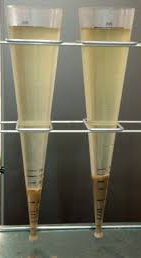
\includegraphics[scale=0.7]{ImhoffCone}\\
			      		Imhoff Cone\\
			      		\textit{Note the ml markings at the bottom of the cone}
			      		
			      		
			      	\end{center}
		      \end{minipage}
%			      \end{minipage}
			      	\item One factor which affects settleability is the conveyance time of the sewage to the treatment plant. 			
			      	\item The settleable component of the suspended solids will decrease as the sewage becomes more septic due to longer conveyance times.
			\item Influent and effluent total suspended solids are measured to establish the overall treatment and individual process efficiencies.  
			\item Volatile solids measurements before and after biological processes such as secondary treatment and digestion provide information on the process efficiency.\\
		\end{itemize}

% 			\end{enumerate}
	\subsubsection{Summary of Wastewater Solids}\index{Summary of Wastewater Solids}		
% 			\begin{snugshade*}
% 				\item \noindent\textsc{Summary of Wastewater Solids}
% 			\end{snugshade*}
			\begin{itemize}
				\item Solids in wastewater can be categorized as dissolved or suspended
				      \begin{itemize}
				      	\item Suspended solids can be further categorized as settleable or unsettleable
				      \end{itemize}
				\item Solids can also be categorized as organic (aka: volatile) or inorganic (aka: fixed)
				\item Colloidial particles are small sized particles some of which pass through the filter and accounted as part of dissolved solids
				\item TSS - Total Suspended Solids are the solids that are captured on the filter paper upon filtration of the wastewater sample.  
				\item Wastewater samples typically analyzed for TSS include:  plant, primary and secondary processes - influent and effluent.  TSS is reported in mg/l
				\item TS - Total Solids are solids content of sludge.  TS of sludge is established by drying a preweighed quantity of sludge in an oven and is typically reported as \% solids - which is how many parts (by weight) of solids per 100 parts (by weight) of sludge.
				\item Volatile solids are solids that are removed when the solids are incinerated at 550C.  The solids that remain after incineration are fixed or non-volatile or inorganic solids.
			\end{itemize}
	\subsubsection{Wastewater Solids Content}\index{Wastewater Solids Content}			
% 			\begin{snugshade*}
% 				\item \noindent\textsc{Typical influent wastewater contains:}
% 			\end{snugshade*}
			\begin{itemize}
				\item Less than 0.1\% total solids.  Total solids concentration in typical wastewater is about 750mg/l
				\item The total solids are 50\% organic (volatile) and 50\% inorganic (fixed)
				\item Of the total solids, dissolved solids constitute about 70\% of the solids and the remaining 30\% solids are suspended solids
				\item 40\% of the dissolved solids are volatile the remaining 60\% are fixed
				\item 70\% of the suspended solids are volatile and the remaining 30\% are fixed
			\end{itemize}
			% \clearpage\thispagestyle{empty}
			\begin{figure}[!htbp]
			\vspace{2cm}
				\begin{center}
					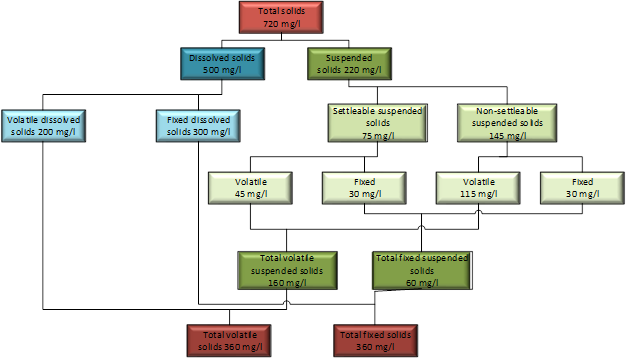
\includegraphics[scale=0.8]{WastewaterSolids}\\
					\caption{Typical Wastewater Solids Concentrations}
				\end{center}
				\end{figure}
% % 			\end{enumerate}
				
\subsection{Nutrients}\index{Nutrients}	
% 			\begin{snugshade*}
% 				\item \noindent\textsc{Nutrients}
% 			\end{snugshade*}	
			\begin{itemize}
				\item Plant nutrients - nitrogen and phosphorous, present in wastewater effluent discharge, promote growth of plant and algal matter in the receiving waters causing destruction of the normal aquatic life mainly due to oxygen depletion - eutrophication.
				      
				\item Because of the potential impacts of the presence of these nutrients in wastewater effluent on the receiving waters,  limits on the levels of these nutrients is typically stipulated in the treatment plant's wastewater discharge permit.
				      
				\item Typically, conventional secondary treatment processes are designed primarily remove the organics from the wastewater.  Secondary treatment process designed to additionally remove nutrients is deemed as tertiary or advanced treatment is termed as Biological Nutrient Removal (BNR).
			\end{itemize}
	\subsubsection{Nitrogen}\index{Nitrogen}				
% 			\begin{enumerate}%@@@@@@@@@@@@@@@@@@%
% 				\definecolor{shadecolor}{RGB}{220,220,220}
% 				\begin{snugshade*}
% 					\item \noindent\textsc{Nitrogen}%@@@@@@@@@@@@@@@@@@%
% 				\end{snugshade*}

	\textbf{Forms of nitrogen:}\\	
% 				\begin{itemize}
% 					\item Forms of nitrogen:\\
					      \begin{itemize}
					      	\item About 60\% of nitrogen in wastewater is present as ammonia nitrogen (about 60\%).  The ammonium nitrogen is present either in the form of ammonia (NH$_3$ ) or as ammonium (NH$_4^+$ ) ion.   These two forms can rapidly change from one to the other depending on pH and temperature.  Under low pH (acidic) or neutral conditions – pH less than or equal to 7, ammonia exists mostly as ammonium.  Ammonia becomes the dominant form as the pH increases to 8 and beyond.
					      	\item The other dominant form of nitrogen, about 40\% of the total nitrogen is as organic nitrogen
					      	\item Nitrogen measured as Total Kjeldahl Nitrogen (TKN) which is the sum of the organic nitrogen and the ammonia nitrogen concentrations.  Total inorganic nitrogen is the total concentration of ammonia nitrogen, NO3-, and NO2-.   Table provides the concentrations and forms of nitrogen in wastewater.
					      \end{itemize}
					      \setlength{\arrayrulewidth}{0.7mm}
					      \setlength{\tabcolsep}{8 pt}
					      \renewcommand{\arraystretch}{0.8}
					      \begin{center}
					      \begin{figure}[!htbp]
					      	\noindent \begin{tabular}[!htbp]{ |p{6cm}|p{2.0cm}|p{2.5cm}|p{2.cm}|}
					      	\hline
					      	\multicolumn{4}{|c|}{\textbf{Forms of Nitrogen in Wastewater}} \\
					      	\hline
					      	%\thead{A Head} & \thead{A Second \\ Head} & \thead{A Third \\ Head} \\
					      	%\hline%
					      	
					      	\hspace{1.8 cm}Forms of Nitrogen & \hspace{0.25 cm} Formula & \hspace{.4 cm} Found in & \hspace{.4 cm} Typical \newline \hspace{.2 cm}Concentration\\
					      	\hline
					      	\small Ammonia/Ammonium & \small NH$_3$/NH$_4^{\enspace +}$ &  \small Influent wastewater & 30-50 mg/l\\
					      	
					      	Total Kjeldahl Nitrogen \newline  \small (Ammonia/Ammonium + Organic Nitrogen) &  \small TKN &  \small Wastewater \newline  \small effluent  & 30-60 mg/l \\
					      	
					      	\small Total Inorganic Nitrogen \newline  \small (Ammonia/Ammonium + Nitrite + Nitrate) & \small TIN &  \small  Wastewater \newline  \small effluent  & 1-40 mg/l \\
					      	
					      	\small Nitrate  & $NO_3^{\enspace -}$ &  \small Nitrified effluent &  \small 1-35 mg/l \\
					      	
					      	\small Nitrate  &  $NO_2^{\enspace -}$ &  \small Partially nitrified effluent &  \small 0.1-2 mg/l \\
					      	
					      	\hline
					      	\end{tabular}
					      	\caption{Forms of Nitrogen}
					      	\end{figure}
					      \end{center}
					      
		\subsubsection{Phosphorous}\index{Phosphorous}			
		\textbf{Forms of phosphorous:}\\
					      \begin{itemize}
					      	\item The principal forms are organically bound phosphorus, polyphosphates, and orthophosphates.
					      	\item Organically bound phosphorus originates from body and food waste and, upon biological decomposition of these solids, is converted to orthophosphates. 
					      	\item Polyphosphates originate from synthetic detergents and are hydrolyzed to orthophosphates. Thus, the principal form of phosphorus in wastewater is assumed to be orthophosphates, although the other forms may exist. Orthophosphates consist of the negative ions PO$_4$$^{3-}$, HPO$_4$$^{2-}$, and H$_2$PO$_4$ $^-$.  These may form chemical combinations with cations (positively charged ions).
					      \end{itemize}

\subsubsection{Oil and Grease}\index{Oil and Grease}	
			Fats, oil and grease in wastewater originate from homes, food establishments and industries.
			\begin{itemize}
				\item Oil and grease content of wastewater is established in the laboratory by extracting it with a solvent - \textit{n}-hexane.  The concentration of oil and grease is reported in mg/l and typical oil and grease content of wastewater ranges from 80 - 120 mg/l
				\item Presence of excessive oils and grease could potentially impact the secondary treatment process
				\item Oils and grease are removed as floatables in primary treatment and sent with the sludge to the digesters
			\end{itemize}

\section{Wastewater Properties and Parameters} \index{Wastewater Properties and Parameters}
			
		Laboratory and field tests are conducted to measure parameters which are critical for monitoring and controlling treatment.  The following are the key parameters that are measured.	
			
\subsection{pH}\index{pH}	
			\hl{pH is a measure of the hydrogen ion (H$^+$) content or the acidity or basicity of a solution.}  pH impacts the chemical and micribiological elements of wastewater treatment processes and thus pH measurement and control is critical.
			\begin{itemize}
				\item Pure water dissociates into equal concentration of hydrogen ions and hydroxide ions:\\ 
				      $H_2O \rightarrow H^+ + OH^-$.
				\item The H$^+$ are responsible for acidic properties and the OH$^-$ ions for the basic properties.  
				\item pH is the inverse of H$^+$ concentration; pH increases when the concentration of H$^+$ decreases relative to the concentration of OH-. 
				\item pH scale ranges from 0 – 14. When the concentration of both H$^+$ and OH$^-$ are equal, as in pure water, it is considered neutral and its pH is 7.0.  \item If the pH of a sample solution is below 7.0, the sample is termed acidic and is alkaline or basic if its pH is above 7.0. 
				\item Each change of 1 pH unit represents a 10 fold change in concentration.  For example, a sample with a pH of 2.0 is 1000 times more acidic than a sample with a pH of 5.0. 
				\item pH is measured by an electrode that is sensitive only to H$^+$ or using a pH strip which is essentially an adsorbent paper which is pre-impregnated with chemicals which change color under different H$^+$ concentrations.
				\item Most organisms involved in biological wastewater treatment processes do well within a a narrow range of pH near neutral (pH of 7).			
			\end{itemize}
			
\subsection{Oxidation Reduction Potential (ORP)}\index{Oxidation Reduction Potential (ORP)}			
			\begin{itemize}
				\item ORP measurements are common in wastewater process control for monitoring conditions and process efficiency
				\item ORP is measured in milivolts (mV) using a probe\\
				\item ORP is a measure of the potential of oxidation/reduction – electron transfer, based chemical reactions to occur 
				\item If the measured ORP value (in mV), is positive it indicates an environment where oxidation will occur and if negative, an environment where reduction reactions will occur
				\item Higher positive value indicates a stronger oxidative environment and likewise, a lower (more negative) ORP value indicates a stronger reductive environment 
				\item For example, during chlorine disinfection, which is an oxidation process, the wastewater will exhibit a positive ORP.  Stronger the oxidative power of chlorine, higher will be the wastewater ORP value
				\item All living matter, including microbes depend upon respiration to generate energy and respiration involves series of chemical oxidation-reduction reactions 
				\item Bacteria grow and thrive only in specific chemical - oxidative-reductive environments which support its inbuilt metabolic pathways
				\item Aerobic bacteria need molecular oxygen as the terminal electron acceptor as part of its cellular respiration proces.  Bacteria adapted to exist in an environment where molecular oxygen is not present (anoxic and anaerobic), rely on electron acceptors such as NO$_3^-$ (denitrification), SO$_4^-$ (sulfide formation) and carbon (methane formers in anaerobic digestion)
				\item Aerobic bacteria responsible for cBOD removal in the secondary treatment process would be inhibited or wiped-out if the wastewater oxidation potential dropped and become reductive.  Likewise, if the wastewater in the sewer pipes which is normally of reductive (negative ORP)  was to become oxidative because of aeration (dissolving oxygen) it would cease the hydrogen slufide activity of the anaerobic bacteria
				\end{itemize}
		
			\setlength{\arrayrulewidth}{0.6mm}
			\setlength{\tabcolsep}{8 pt}
			\renewcommand{\arraystretch}{1.2}
			\begin{center}
			\begin{table}[!htbp]
				\begin{tabular}{ |p{9.5cm}|p{4.0cm}|}
					\hline
					\multicolumn{2}{|c|}{\textbf{Typical Wastewater Process ORPs}} \\
					\hline
					
					\hline
					\small Clorine disinfection & \small +650 to +700 mV  \\
					\small Nitrification & \small +100 to +350 mV   \\
					\small Biological phosphorous removal & \small +20 to +250mV        \\
					\small Activated sludge	cBOD degradation with free molecular oxygen & \small +50 to +250 mV  \\
					\small Denitrification                                              & \small +50 to -50 mV   \\
					\small Influent wastewater                                          & \small - 200 mV  \\ 
					\small Sulfide formation                                & \small -50 to -250 mV  \\
					\small Anaerobic Digestion: Acid formation (Acidogenesis)           & \small -100 to -225 mV \\
					\small Biological phosphorous removal & \small -100 to -250 mV \\
					\small Anaerobic Digestion: Methane production  (Methanogenesis)     & \small -75 to -400 mV  \\
					\hline
				\end{tabular}
	\end{table}			
			\end{center}
			
\subsection{Alkalinity}\index{Alkalinity}	
			\begin{itemize}
				\item \hl{Alkalinity is the ability of a water to neutralize acids.}  
				\item During certain wastewater treatment processes including anaerobic digestion, acids are generated as a result of microbiological activity.  The bacteria and other biological entities which play an active role in wastewater treatment are most effective at a neutral to slightly alkaline pH of 7 to 8.  In order to maintain these optimal pH conditions for biological activity there must be sufficient alkalinity present in the wastewater to neutralize acids generated by the active biomass.
				\item This ability to maintain the proper pH in the wastewater as it undergoes treatment is the reason why alkalinity is so important to the wastewater industry.
				\item The alkalinity is due to the presence of acid neutralizing bases in the water including the hydroxyl (OH$^-$), carbonate (CO$_3$$^-$) and bicarbonate (HCO$_3$$^-$)  ions.  These ions are of mineral origin and are also formed from carbon dioxide which comes from the atmosphere and from the microbial decomposition of organic material.  The resistance to pH change of the water will continue until all the alkalinity contributing ions are neutralized.  
				\item The pH of a water serves as a guide to the types of alkalinity present in the water but is unrelated to the alkalinity content of a water.  Important Note:  Alkalinity is a measure of the ability to neutralize acids whereas a solution is termed alkaline (or basic) if its pH greater than 7. 
				\item Alkalinity is expressed as milligrams per liter of CaCO$_3$
			\end{itemize}
			
\subsection{Dissolved Oxygen}\index{Dissolved Oxygen}	
			\begin{itemize}
				\item Dissolved oxygen (DO) is the concentration of oxygen dissolved in the wastewater sample and is typically measured in the field using a DO probe.  A titration based Winkler Test is used in the laboratory
				\item The \hl{presence of oxygen indicates an aerobic environment} where dissolved, free oxygen is available for aerobic microorganisms to live, BOD removal in the activated sludge process occurs as a result of the activity of aerobic bacteria.  The absence of DO indicates that the environment or condition is either anoxic or anaerobic.  
				\item \hl{In an anoxic environment, free oxygen is not present, but oxygen is available from its combined  forms - nitrate (NO$_3$ $^-$) and sulfate (SO$_4$ $^-$)} for the the consumption of microorganisms.  Example of an anoxic process is denitrification.  In denitrification, the anoxic bacteria in the presence of food (cBOD) consume the combined oxygen in nitrates (NO$_3$ $^-$ ) and convert it to nitrogen gas.
				\item \hl{The complete absence of oxygen including free and combined oxygen is an anaerobic environment.}
				\item Microorganisms are termed as obligate aerobes if they cannot survive without free oxygen.  Facultative aerobes are microorganisms which can survive in both aerobic and anaerobic environments.  
			\end{itemize}
			
\subsection{Microbiological testing and monitoring}\index{Microbiological testing and monitoring}	
			
			Microbes play a critical role in wastewater treatment.  
			\begin{itemize}
				\item Heterotrohic (organisms that consume organic material) microbes are responsible for the biological wastewater treatment processes - secondary treatment process, digestion and nutrient removal; and
				\item Pathogens - agents that cause disease are present in wastewater effluent.
			\end{itemize}
Microbiological testing and monitoring is conducted as part of the wastewater treatment typically for the following:
\begin{enumerate}[1.]
				
				\item Microbiological testing related to monitoring and troubleshooting biological wastewater treatment\\
				
				Microbes involved in biological wastewater treatment processes include:\\
				\begin{itemize}
					\item Fungi - Filamentous fungi occasionally bloom in activated sludge processes due to low pH or nutrient deficiency and cause problems with the settleability.
					\item Protozoa - Protozoas play a important role in the secondary treatment process.  Common protozoas in the activated sludge process include:
					      \begin{itemize}
					      	\item Amoeba
					      	\item Flagellate
					      	\item Cilliate
					      \end{itemize}
					\item Rotifers
					\item Nematodes
					\item Bacteria - Bacteria is the predominant microorganism responsible for the biological wastewater water treatment.  
				\end{itemize}
				\begin{itemize}
					\item The effectiveness of the biological wastewater treatment processes is primarily due to the presence of a microbial ecosystem with a right balance of populations of different microbial species.
					\item Methods used for monitoring the microbial composition include direct monitoring using a light microscope to see which and how many of the different microbial species are present - typically used for activated sludge process.
					\item Indirect method includes monitoring other parameters such as pH and alkalinity which are influenced by microbiological activity.
					\item The microbial monitoring ensures process stability and helps identify potential process upset conditions caused by changes to the microbial population due to other external factors - toxicty, organic loading, temperature etc.
				\end{itemize}

\item Microbiological testing related to monitoring and controlling pathogens in treated wastewater effluent\\

	
				Pathogens in wastewater belong to the following groups:
				\begin{itemize}
					\item Bacteria:  Although, bacteria is present in large numbers in feces, pathogenic or bacteria are present only because of an infection and this pathogenic bacteria can potentially spread the infection to other healthy individuals.  Disease spread by pathogenic bacteria include diarrhea, cholera and typhoid among many others.
					      
					\item Viruses: A large number of viruses may infect humans and are present in feces.  These include enteroviruses (including polioviruses), hepatitis A virus, reoviruses and diarrhea-causing viruses (especially rotavirus).
					      
					\item Protozoa:  Many species of protozoa can infect humans and cause diarrhoea and dysentery. Girardia which casues diarrheal illness is an example of a protozoan pathogen
					      
					\item Helminths:  These are parasitic worms that can infect humans and are transmitted to others through its eggs or larval forms
					      
				\end{itemize}
				
				\begin{itemize}
					\item As one of the main reasons for treating wastewater is to protect public health, microbiological/pathogen testing of the wastewater effluent and the surface water impacted by the wastewater discharge is conducted to meet the requirements of a wastewater discharge permit, to monitor the pathogen impact of treated wastewater discharge and assess the level of contamination of a public body of water.
					\item The bacteriological tests involves detection and quantification of one or more of the following bacteria:  total coliforms, fecal coliforms, E. Coli, and Enterococcus.  
					      \begin{itemize}
					      	\item The main reason why these bacteria such as coliforms and enterococcus are used \hl{as it is not practical to detect and quantify all pathogens associated with wastewater.}  
					      	\item These selected bacteria originate from feces and indicate fecal contamination and thus serve as an indicator organisms for pathogens of wastewater origin.  
					      	\item Also, they are abundant, potentially less harmful, and easy to detect.  E. coli has been shown to be a better predictor of the potential for impacts to human health and therefore many newer wastewater discharge permits require E. Coli testing in lieu of fecal coliform testing requirements.
					      \end{itemize}
					\item The microbiological test sample is always collected as a grab in a clean, sterile borosilicate glass or plastic bottle containing sodium thiosulfate. 
					      \begin{itemize}
					      	\item Sodium thiosulfate is added to remove residual chlorine which will kill coliforms during transit. 
					      	\item If the sample is not preserved or maintained under proper conditions until the test is conducted in the laboratory, the test would provide erroneous results.
					      	\item Samples must be refrigerated if they cannot be analyzed within 1 hour of collection and must be handled with care to prevent contamination and adverse conditions such as prolonged exposure to direct sunlight.
					      	\item The maximum holding time for state or federal permit reporting purposes is 6 hours. 
					      \end{itemize} 
					\item As it is not possible to exactly quantify the number of bacteria present, a statistical based - \hl{Most Probable Number (MPN)} approach is utilized.  The methods for wastewater bacteriological tests include:  multiple-tube fermentation technique, membrane filtration and quanti-tray testing. 
				\end{itemize}
			\end{enumerate}

\subsection{Specific Gravity}\index{Specific Gravity}				
			\begin{itemize}
				\item Specific gravity is a term to express the weight of a solution with respect to that of water
				\item Water weighs 1 kg/L or 8.34 lbs/gallon or 62.4 lbs/ft$^3$
				\item A solution with a specific gravity of 1.2 will weigh 1.2 times the same volume of water.  1 L of that solution will weigh ( 1.2 kg )/L  or  ( 1.2*8.34=10lbs )/gallon.
				\item Typically wastewater and the associated unthickened sludge, for all practical purposes is assumed to have a specific gravity of 1 - implying 8.34 lbs/gallon.
				\item Specific gravity is typically used for calculations related to chemicals used in wastewater treatment.
			\end{itemize}

\section{Wastewater Sampling} \index{Wastewater Sampling}		
		\begin{itemize}
			\item Field or laboratory measurement of a certain parameter is critical in wastewater treatment operations to obtain information about wastewater characteristics in order to either characterize a wastewater stream, or to monitor a treatment process or for permit compliance.  
			\item A sample is a small part of the whole representing the whole.  Thus, a sample needs to be such that it truly represents the entire population – which in a wastewater operations could be either a wastewater stream, wastewater solids or a chemical used.
		\end{itemize}
		
\subsection{Sampling Methods}\index{Sampling Methods}
\subsubsection{Grab Samples}\index{Grab Samples}
				\begin{itemize}
					\item A grab sample is a sample collected at a specific spot at a site over a short period of time.  
					\item Grab sampling allows for instantaneous analysis of parameters such as pH, dissolved oxygen, chlorine residual, temperature and other parameters which change rapidly with time.
					\item A grab sample represents a snapshot of space and time of a process stream.
					\end{itemize}
\subsubsection{Composite Samples}\index{Composite Samples}
				\begin{itemize}
					\item A composite sample is a collection of discrete samples are combined over a certain period or space and therefore represent the average performance of a wastewater treatment plant or a process during the collection period.\\  
					\item Composite sampling can be either based on:
					      
					      1. constant time interval (time proportioned sampling)\\
					      2. constant wastewater volume interval (flow-proportioned sampling), and\\
					      3. treatment process space - includes samples taken at different depths\\
					      
					\item Composite samples are typically collected using automated samplers which can be programmed to collect samples at pre-established time intervals – for time proportional sampling.
					\item Time and space composite samples are collected by adding equal volumes of samples collected from different times or locations.  
					\item Flow proportional composite samples comprise of volume of each subsample based on flow.\\  
				\end{itemize}
				
			\begin{center}
				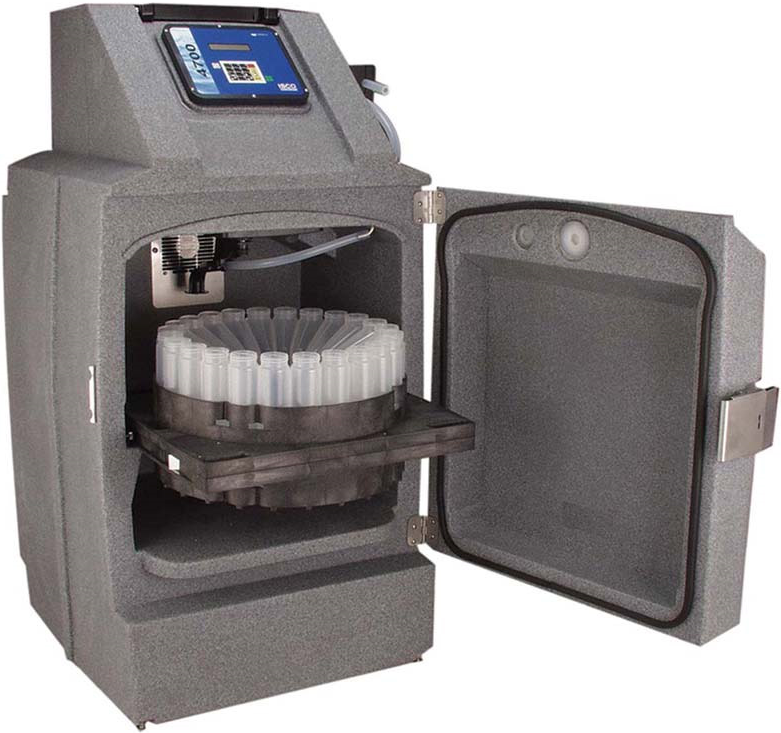
\includegraphics[scale=0.2]{Autosampler} \hspace{2cm} 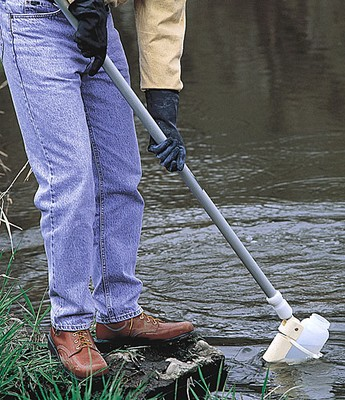
\includegraphics[scale=0.37]{Grabsampler}\\
			\end{center}
			\hspace{2.3cm} Automated Sampler \hspace{2.0cm} \parbox{\textwidth}{Grab Sampling Using a Long Handle Dipper}\\

\subsubsection{Sampling Precautions and Protocols}\index{Sampling Precautions and Protocols}
			\begin{itemize}
				\item Samples should represent the major portion of the process or the process stream and should be taken from places where the mixing is thorough, avoiding dead spots and areas of heavier or lighter loadings. 
				\item The collected sample is invariably exposed to conditions very different from the original source and is subject to change due to chemical and microbiological activity.  
				\item Thus, in order to ensure integrity of sample, sample preservation techniques specific to the analysis to be performed is needed.  
				      \begin{itemize}
				      	\item The preservation technique should not only allow for stabilizing the parameter to be analyzed, it should also not interfere with the analyses.  
				      	\item The common preservation techniques involve use of proper containers, temperature control, addition of chemical preservatives, and observance of the recommended maximum sample holding time.
				      \end{itemize}
			\end{itemize}
			
\subsubsection{Bacteriological Sampling}\index{Bacteriological Sampling}
\begin{itemize}
\item Always collected as a grab
\item A clean, sterile borosilicate glass or plastic bottle containing sodium thiosulfate is used. Sodium thiosulfate is added to remove residual chlorine which will kill coliforms during transit. If the sample is not preserved or maintained under proper conditions until the test is conducted in the laboratory, the test would provide erroneous results
\item Samples must be refrigerated if they cannot be analyzed within 1 hour of collection
\item Samples must be handled with care to prevent contamination and adverse conditions such as prolonged exposure to direct sunlight
\item Maximum holding time for state or federal permit reporting purposes is 6 hours
\end{itemize} 

\subsection{Data Reporting}\index{Data Reporting}	
		\begin{itemize}
			\item Arithmetic mean is typically calculated for reporting data where multiple samples have been collected and analyzed for the same process stream at different times and for reporting average value over a certain time period – daily, monthly etc.\\ \item Arithmetic mean mathematically is calculated by adding all the result values and dividing by the total number of data points.\\
		\end{itemize}
		Mathematically the arithmetic mean is represented as:\\
		$$\bar{x}=\frac{\sum_{i=1}^{n} x^i}{n} = \frac{x_1+x_2+x_3...x_n}{n}$$
		For example:\\
		Arithmetic mean of the following set of data points:  200, 304, 250, 400 is calculated as:\\
		\vspace{10pt}
		Arithmetic Mean = $\frac{200 + 302 + 250 + 400}{4}= 288$\\
		\vspace{10pt}
		For data sets for analysis such as fecal coliform could include values which vary by several orders of magnitudes, using the arithmetic mean to report the average value is not appropriate as the lower or higher values would bias the calculated mean.\\
		\vspace{10pt}
		For example, consider a data set with values:  260, 300, 500, 5,000, 320 and 200.\\
		\vspace{10pt}
		The arithmetic mean = $\frac{260+300+500+5,000+320+200}{6} = 3,444$\\
		Here the 5000 value completely skews the arithmetic mean.
		
		Therefore, for such tests, the geometric mean calculation is used for reporting the average value.\\
		
		
		Mathematically a geometric mean is represented as:\\
		$$\Bigg(\prod_{i=a}^n\Bigg)^{\frac{1}{n}}=\sqrt[n]{a_1*a_2*a_3...a_n}$$
		 
		Calculation method:\\
		1.	Find the product of all the data points (analogous to first calculating the sum of all the data points when calculating the arithmetic mean)\\
		260*300*500*5,000*320*200 = 12,480,000,000,000,000\\
		2.	Raise the product to the inverse of the number of data points\\
		(*Using the power function of a scientific calculator)\\
		Here n (\# data points) = 6 $\implies$ geometric mean = $(12,480,000,000,000,000)^{\frac{1}{6}}   = 482$

\section{Laboratory Analysis}\index{Laboratory Analysis}

		\subsection{BOD Analysis}\index{BOD Analysis}		
\begin{itemize}
\setlength\itemsep{1em}

\item The Biochemical Oxygen Demand (BOD) test estimates the amount of biodegradable material present by measuring the amount of oxygen used by the bacteria to break down the organic waste in the sample incubated at 20 deg. C over a five-day period . The BOD test provides an indication on the strength of wastewater in terms of how much oxygen could be depleted if that wastewater was introduced into another receiving water.  Complete stabilization of a sample may require a period of incubation too long for practical purposes; therefore, 5 days has been accepted as the standard incubation period.

\item As the regular BOD test includes estimation of oxygen nitrifying bacteria consumes in the process of converting inorganic forms of ammonia and nitrogen to nitrite and nitrate, its value represents oxygen used for removing both, organic material and nitrogenous matter.  As this BOD value does not quite represent the organic strength of the wastewater, the normal BOD test is modified by introducing a chemical inhibitor - 3 mg of 2-chloro-6-(trichloro methyl) pyridine (TCMP), which suppresses the growth of the nitrogenous bacteria so that the resultant BOD measured represents the oxygen depletion associated with the depletion of the organic matter only.  This is the Carbonaceous biochemical oxygen demand or cBOD. \\
\vspace{0.4cm}
\textbf{Thus tBOD = nBOD + cBOD}

\item Wastewater BOD measurement involves testing a sample set consisting of several sample dilutions along with a "Blank".  "Blank" is a sample with only the dilution water with no wastewater added. \\


\item The dilutions are made based upon the expected BOD concentration of the sample.  Using the final dilution volume of 300 ml, the initial sample volume can be estimated using the formula:\\

\textbf{$Sample \enspace Volume (ml) = \dfrac{\Big[Oxygen \enspace Depletion \Big(\dfrac{mg}{l}\Big)\Big]}{Anticipated \enspace BOD \Big(\dfrac{mg}{l}\Big)}*300 \enspace ml$}\\

\item For example, if testing an influent wastewater BOD with an expected BOD value of 250 mg/l, a range of sample volumes for dilution around sample volume of $\dfrac{4\dfrac{mg}{l}}{250 \dfrac{mg}{l}}*300 \enspace ml$=5ml.\\
\vspace{0.4cm}
\item The data obtained for each of the dilutions after the 5-day incubation period must meet the following criteria for the sample value to be acceptable for calculating the BOD.\\
\vspace{0.4cm}

\begin{enumerate}[1.]
\setlength\itemsep{1em}

\item A residual DO of at least 1 mg/L,
\item A DO depletion of at least 2 mg/L
\end{enumerate}
\vspace{0.4cm}
\item Additionally, the whole sample set is rejected if the Blank shows an oxygen depletion of >0.2mg/l.\\
\vspace{0.4cm}
\item BOD is calculated for each sample dilution value using the following formula:\\
\vspace{0.4cm}
\textbf{$BOD \Big(\dfrac{mg}{l}\Big) = \dfrac{Initial \enspace DO - DO \enspace Day \enspace 5}{Sample \enspace Volume \enspace (ml)}*300 \enspace ml$}\\



\end{itemize}
\vspace{0.4cm}
\subsection{Wastewater solids}\index{Wastewater solids}

	\subsubsection{Total (TSS) and Volatile (VSS)}\index{Total (TSS) and Volatile (VSS)}
\begin{itemize}
\setlength\itemsep{1em}
					\item A known volume of wastewater sample is filtered through a pre-weighed filter paper
					\item The suspended solids will be retained by the filter
					\item The water with the dissolved solids will pass through the filter
					\item The filter paper with the filter solids is rinsed with distilled water to remove 
					\item The filter paper with the solids is dried in the oven and then weighed
					\item The difference between the weight of the dried filter paper with the solids and the pre-weighed filter paper, measured in mg, will be the suspended solids in: mg per the original quantity of wastewater sample taken.  This value can be converted to give the suspended solids content in mg/l
					\item A filter paper with the dried solids is incinerated in a muffler furnace
					\item The difference in the weight of the solids, before and after incineration is the fixed solids
					\item The difference between the weight of the solids before incineration and the fixed solids is the volatile solids
	\end{itemize}				

\textbf{Total Suspended Solids - TSS}
\vspace{0.4cm}
$TSS \dfrac{mg}{l}=\dfrac{weight \enspace of \enspace solids \enspace \cancel{gms}}{volume \enspace of \enspace sample \enspace \enspace \cancel{ml}}*\dfrac{1000 \enspace \cancel{ml}}{l}*\dfrac{1000 \enspace mg}{\cancel{gms}}$\\
\vspace{0.3cm}
\hspace{1.4cm}$=\dfrac{weight \enspace of \enspace filter \enspace paper  \enspace with \enspace dried  \enspace solids - weight \enspace of \enspace filter \enspace paper}{volume \enspace of \enspace sample \enspace \enspace (ml)}*1,000,000$\\
\vspace{0.4cm}

\vspace{0.4cm}
\textbf{Volatile Suspended Solids - VSS}	
\vspace{0.4cm}

$VSS \dfrac{mg}{l}=\dfrac{weight \enspace of \enspace volatile \enspace solids \enspace \cancel{gms}}{volume \enspace of \enspace sample \enspace \enspace \cancel{ml}}*\dfrac{1000 \enspace \cancel{ml}}{l}*\dfrac{1000 \enspace mg}{\cancel{gms}}$\\
\vspace{0.3cm}
\hspace{1.4cm}$=\dfrac{wt. \enspace of \enspace filter \enspace paper  \enspace with \enspace dried  \enspace solids - wt. \enspace of \enspace filter \enspace paper \enspace incinerated \enspace residue}{volume \enspace of \enspace sample \enspace \enspace (ml)}*1,000,000$\\
\vspace{0.3cm}
$VSS(\%)=\dfrac{weight \enspace (gms) \enspace of \enspace volatile \enspace solids}{100 \enspace gms \enspace total \enspace solids}=\dfrac{gms \enspace volatile \enspace solids}{\cancel{gms \enspace total \enspace solids}}*\dfrac{100 \cancel{\enspace gms \enspace total \enspace solids}}{100 \enspace gms \enspace total \enspace solids}$\\
\vspace{0.3cm}
\hspace{1.5cm}\small{$=\dfrac{wt. \enspace of \enspace filter \enspace paper  \enspace with \enspace dried  \enspace solids - wt. \enspace of \enspace filter \enspace paper \enspace incinerated \enspace residue}{wt. \enspace of \enspace filter \enspace paper  \enspace with \enspace dried  \enspace solids - wt. \enspace of \enspace filter \enspace paper}*100$}\\				

	\subsubsection{Wastewater and Sludge Total \& Volatile Solids}\index{Wastewater and Sludge Total \& Volatile Solids}
\vspace{0.4cm}
\begin{itemize}
\setlength\itemsep{1em}
					\item A certain quantity of wastewater (by volume) or sludge (by weight) is taken in a pre-weighed dish and weighed.  \hl{Note:  the sample is not filtered.}
					\item The dish with the sample is dried in an oven
					\item The difference in the weight of the pre-weighed dish from that of the dish with the dried sample is the total solids
					\item The dried solids are incinerated in a muffler furnace
					\item The difference in the weight of the solids, before and after incineration is the fixed solids
					\item The difference between the fixed solids and the total solids is the volatile solids
					\item Total solids of a sludge sample is reported as a \% of the sludge weight.  A 7\% sludge has 7 lbs of solids for every 100 lbs of sludge.
				\end{itemize}
				
				\hl{For sludge samples, volatile solids is typically reported as the volatile solids fraction in \% of the total solids content of the sludge.  For example, if a 8\% sludge (i.e sludge which has 8\% TS or 80,000mg/l solids), is reported to have 70\% volatile, it means that 70\% of the total solids - 0.7*8\%=5.6\% or 56,000mg/l is the sludge volatile solids content.  \emph{70\% volatile does not meet the sludge has 700,000mg/l volatile solids}}\\	

\vspace{0.4cm}
\textbf{Total Solids - TS}			
\vspace{0.4cm}
$TS(\%)=\dfrac{weight \enspace of \enspace solids \enspace (gms)}{100 \enspace gms \enspace of \enspace sample}=\dfrac{gms \enspace solids}{gms \enspace sample}*100$\\
\vspace{0.3cm}
\hspace{1.2cm}$=\dfrac{weight \enspace of \enspace cruicible \enspace with \enspace dried  \enspace solids - weight \enspace of cruicible}{weight \enspace of \enspace cruicible \enspace with \enspace sample - weight \enspace of cruicible}*100$\\
\vspace{0.4cm}
\textbf{Total Volatile Solids - VS}		
\vspace{0.4cm}
$VS(\%)=\dfrac{weight \enspace of \enspace volatile \enspace solids \enspace (gms)}{100 \enspace gms \enspace of \enspace total \enspace solids}=\dfrac{gms \enspace volatile \enspace solids}{gms \enspace total \enspace solids}*100$\\
\vspace{0.3cm}
\hspace{1.2cm}$=\dfrac{wt. \enspace of \enspace cruicible  \enspace with \enspace dried  \enspace solids - wt. \enspace of \enspace cruicible \enspace incinerated \enspace residue}{wt. \enspace of \enspace cruicible  \enspace with \enspace dried  \enspace solids - wt. \enspace of \enspace cruicible}*100$\\

\newpage
\thispagestyle{empty}
% \begin{landscape}
% \begin{center}
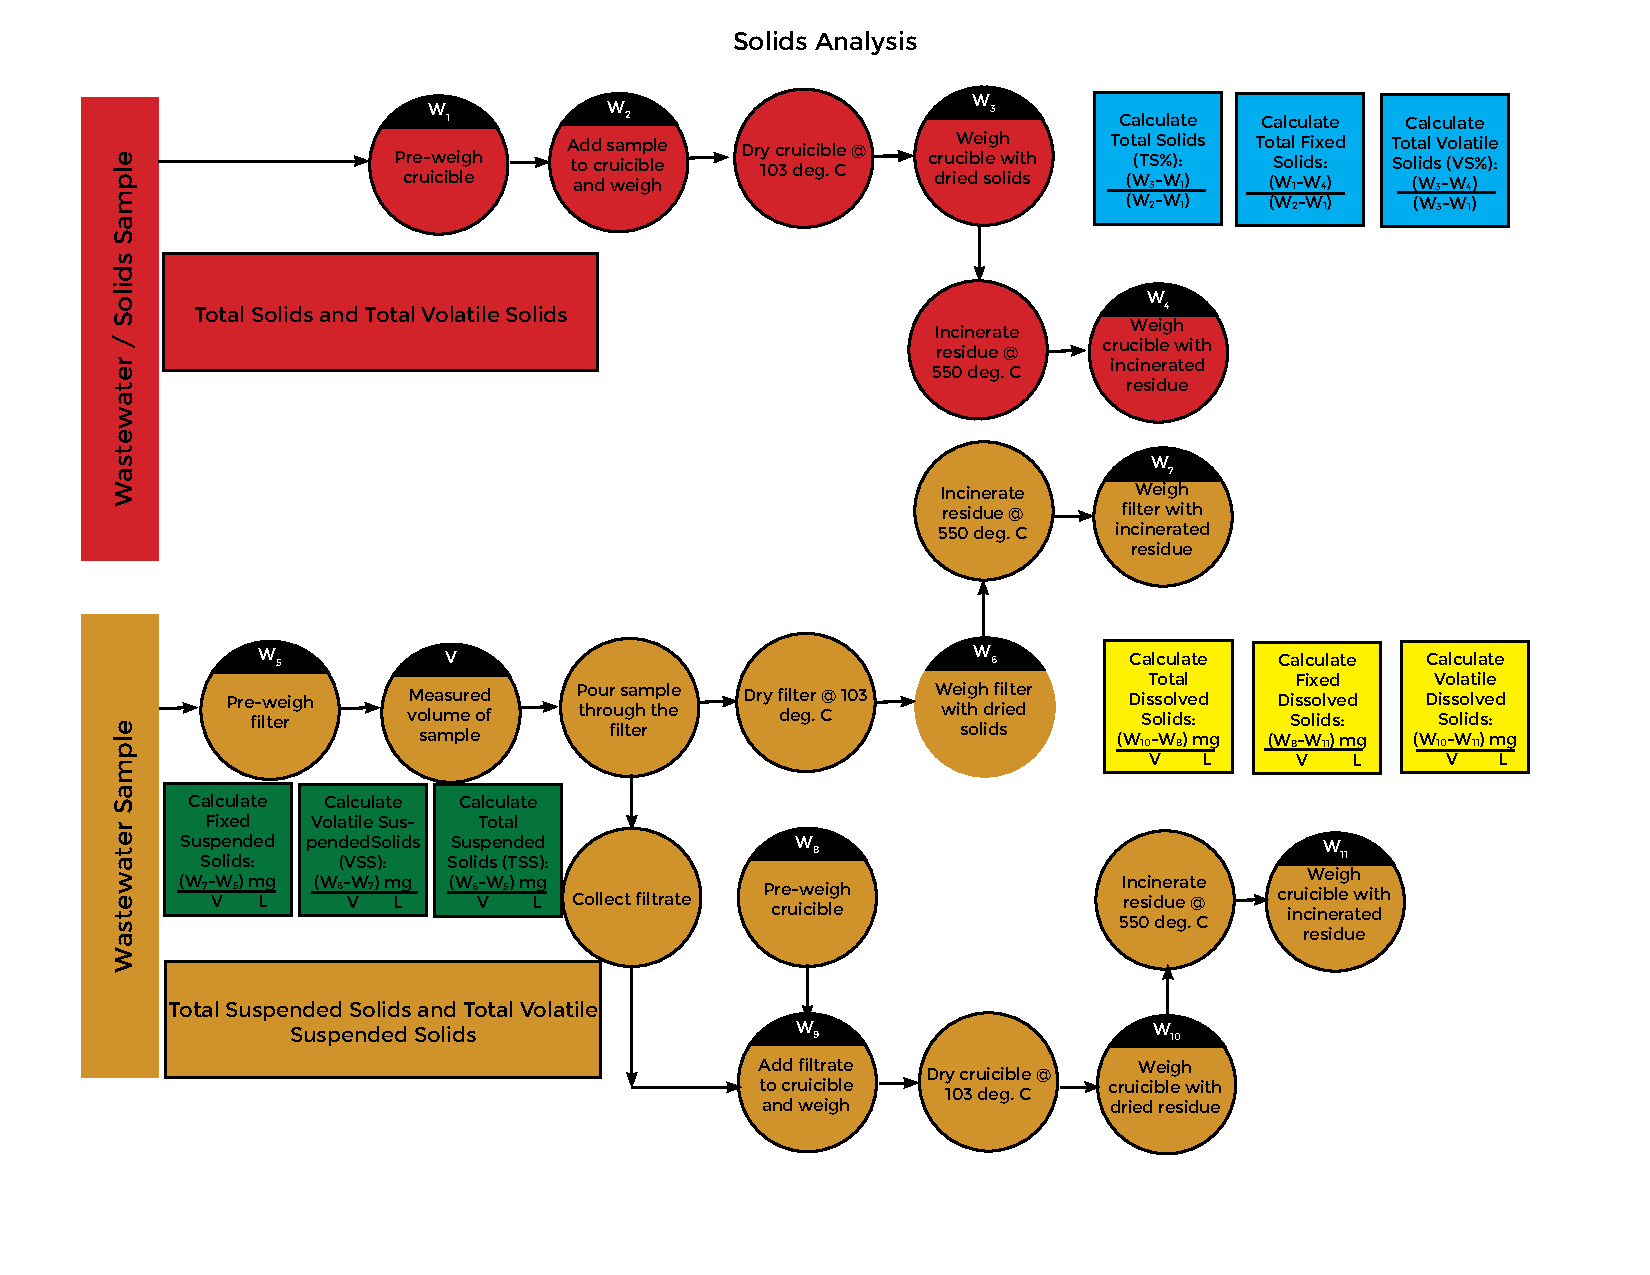
\includepdf[landscape=true]{LaboratorySolidsAnalysis4_01.pdf}
				\newpage
				\thispagestyle{empty}
				\begin{sidewaysfigure}
					\begin{center}
						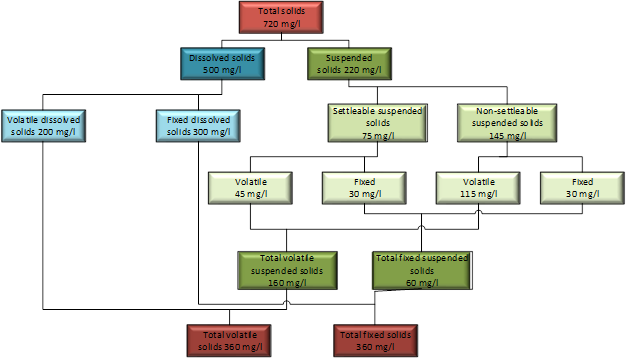
\includegraphics[scale=1.0]{WastewaterSolids}\\
						\caption{Typical Wastewater Solids Concentrations}
					\end{center}
				\end{sidewaysfigure}
%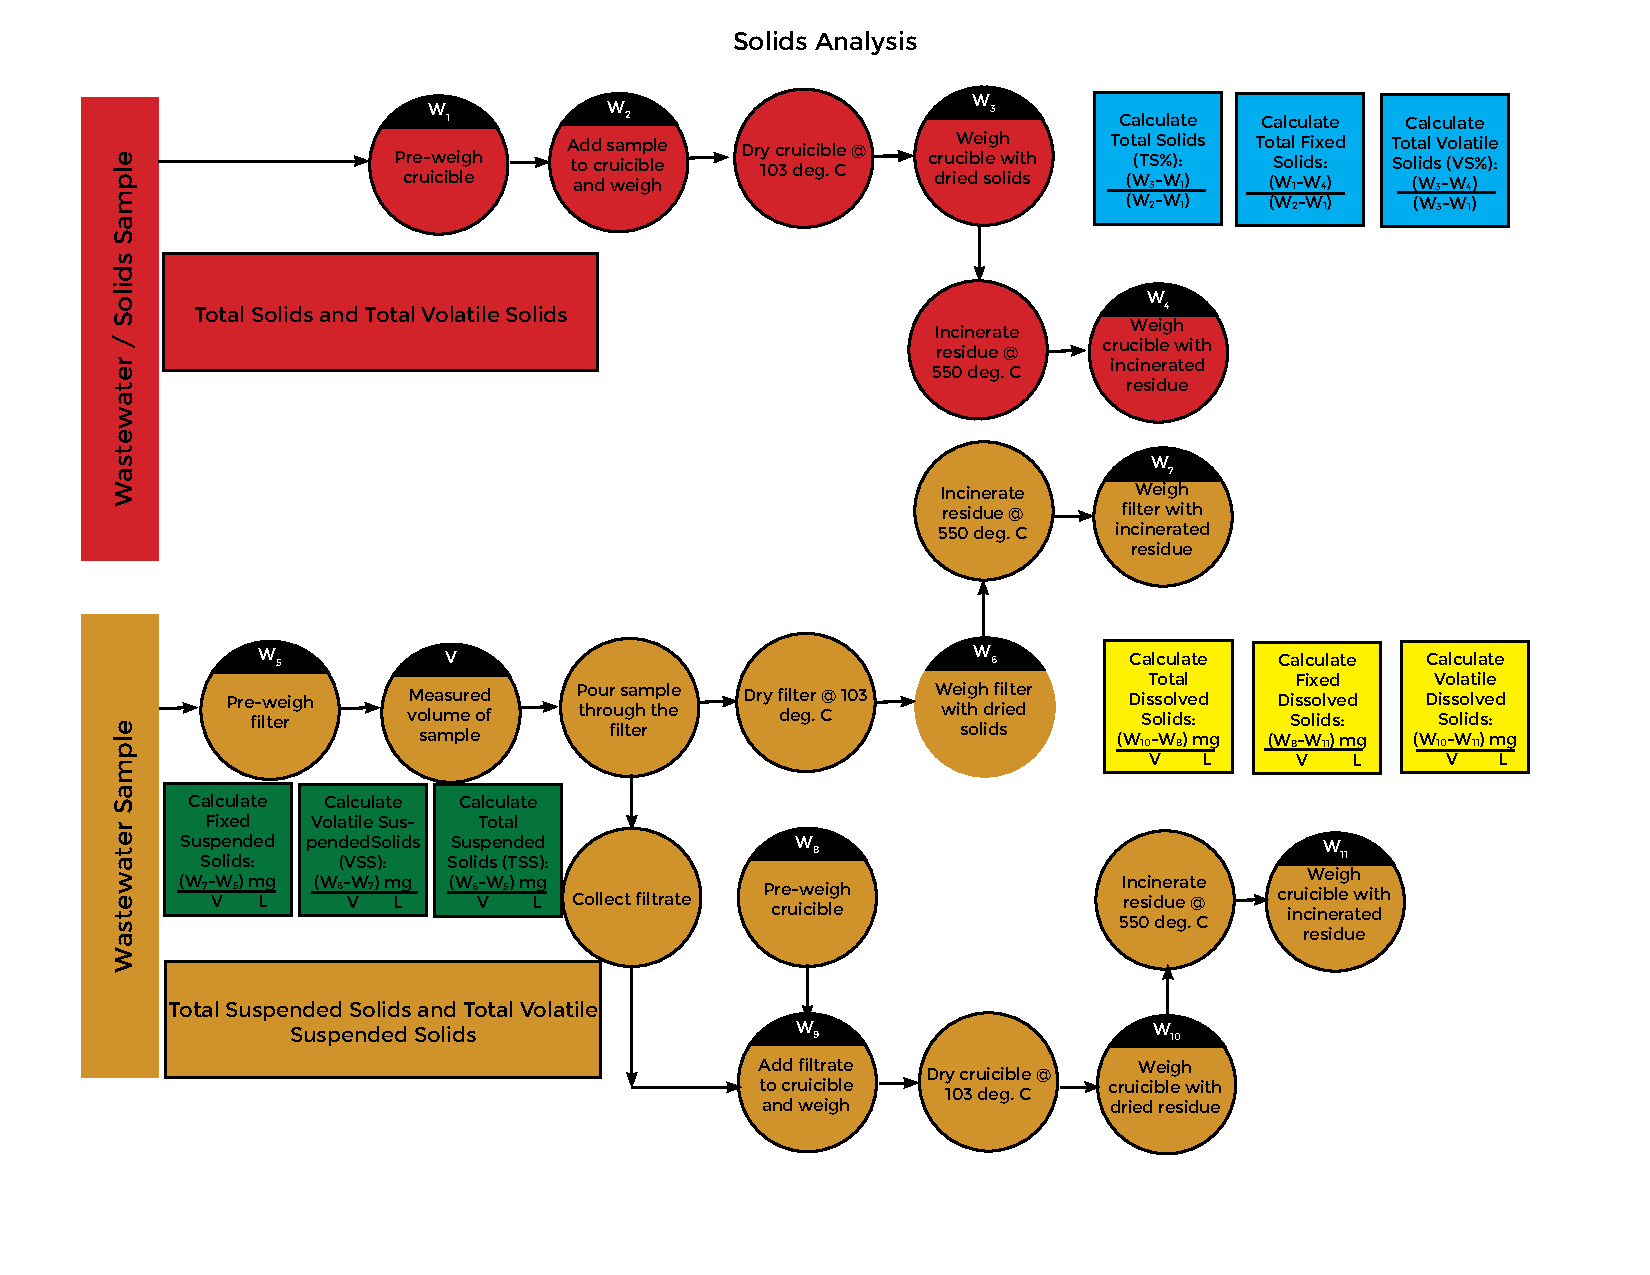
\includegraphics[scale=0.69]{LaboratorySolidsAnalysis4_01.pdf}
% \end{center}
% \end{landscape}
\subsubsection{Sample BOD and solids analysis math problems}\index{Sample BOD and solids analysis math problems}
\begin{enumerate}
\item BOD tests are run on the final effluent from an activated sludge plant with and without the use of a "nitrification inhibitor". Three hundred milliliter bottles (300 ml) are used in these tests. The raw data for these tests are presented below.  What \textbf{percentage of the average total BOD is the average nBOD}?\\
\vspace{0.5cm}
\begin{tabular}{m {4 cm} m {1.5 cm} m  {1.5 cm} m  {1.5 cm} m  {1.5 cm} m {1.5 cm}}
\cline{1-6}
Sample Volume, ml    & 10 & 20 & 30 & 40 & Blank\\
\hline
Initial DO, mg/l 			& 9.0 	& 	8.9 & 8.8  & 9.1 & 9.1\\
Final DO, mg/l 			& 6.9 	& 	4.8 & 2.5 & 1.1 & 9.0
\end{tabular}
\vspace{0.7cm}\\
BOD Test with "inhibitor" added	(cBOD)\\
\vspace{0.5cm}
\begin{tabular}{m {4 cm} m {1.5 cm} m  {1.5 cm} m  {1.5 cm} m  {1.5 cm} m {1.5 cm}}
\cline{1-6}
Sample Volume, ml    & 10 & 20 & 30 & 40 & Blank\\
\hline
Initial DO, mg/l 			& 8.9 	& 	8.9 & 9.0  & 9.0 & 9.1\\
Final DO, mg/l 			& 7.5 	& 	6.2 & 5.0 & 3.3 & 9.0
\end{tabular}
\vspace{0.5cm}\\
Solution:\\
Blanks for both tBOD and cBOD are both <=0.2mg/l - thus sample sets are acceptable\\
\vspace{0.5cm}
\begin{tabular}{m {3 cm} m {2.5 cm} m  {2.5 cm} m  {2.5 cm} m  {2.5 cm} }
\cline{1-5}
Sample Volume, ml    & 10 & 20 & 30 & 40 \\
\hline
tBOD Diff., mg/l    & 2.1 & 4.1 & 6.3 & 8 \\
tBOD, mg/l    & 2.1*300/10 & 4.1*300/20 & 6.3*300/30 & 8.0*300/40\\
    & =63.0 & = 61.5  & = 63.0 & = 60.0 \\
\hline
cBOD Diff., mg/l    & 1.4 & 2.7 & 4.0 & 5.7 \\
cBOD, mg/l    & Reject & 2.7*300/20 & 4.0*300/30 & 5.7*300/40\\
    & Depletion < 2 & = 40.5  & = 40 & = 42.75 \\
\end{tabular}
\vspace{0.5cm}\\

$tBOD (avg) = (63+61.5+63+60)/4=61.9 \hspace{1cm} cBOD (avg) = (40.5+40+42.75)/3=41.1$\\
nBOD = tBOD - cBOD $\implies$ nBOD = 61.9-41.1=20.8 $\implies$ nBOD(\%)=20.8/61.9*100=$\boxed{33.6\%}$
\vspace{0.5cm}
\item Calculate percent total solids and percent volatile solids of a sludge sample given the following data:\\
\begin{tabular}{m {5 cm} m {0.5 cm} m  {3.5 cm}}
Weight of dish &=&  104.55 gms\\
Weight of dish and wet sludge &= & 199.95 gms\\
Weight of dish and dry sludge &= & 108.34 gms\\
Weight of dish and ash &= & 106.37 gms
\end{tabular}\\
\vspace{0.2cm}
Solution:\\
\vspace{0.2cm}
Weight of dish=104.55 gms\\
Weight of dish and wet sludge=199.95 gms\\
Weight of dish and ash = 106.37 gms\\
\vspace{0.2cm}
$ \implies Weight \enspace of \enspace sludge=199.95-104.55=95.40 \enspace gms$\\
$\implies Weight \enspace of \enspace dry \enspace sludge \enspace (solids)=108.34-104.55=3.79 \enspace gms$\\
$\implies Weight \enspace of \enspace volatile \enspace solids=108.34-106.37=1.97 \enspace gms$\\
\vspace{0.2cm}
$Total \enspace solids (TS\%)=\dfrac{gms \enspace solids}{100 \enspace gms \enspace sludge}=\dfrac{3.79}{95.40} \enspace \dfrac{gms \enspace solids}{\cancel{gms \enspace sludge}}*\dfrac{100 \cancel{\enspace gms \enspace sludge}}{100 \enspace gms \enspace sludge}=\boxed{3.97\%}$\\
\vspace{0.2cm}
$Total \enspace volatile \enspace solids (VS\%) =\dfrac{1.97}{3.79} \enspace \dfrac{gms \enspace volatile \enspace solids}{\cancel{gms \enspace total \enspace solids}}*\dfrac{100 \cancel{\enspace gms \enspace total \enspace solids}}{100 \enspace gms \enspace total \enspace solids}=\boxed{52.0\%}$\\


\end{enumerate}

\subsection{Bacteriological Ennumeration}\index{Bacteriological Ennumeration}

\begin{tabular}{|c||l|}
\hline
\multicolumn{1}{|c|}{Pathogen} & \multicolumn{1}{c|}{Disease Caused} \\
\hline
Bacteria: &  \\
\hline\hline
Anthrax & anthrax \\
\hline\hline
Escherichia coli & E. coli infection \\
\hline\hline
Myobacterium & tuberculosis \\
tuberculosis &  \\
\hline\hline
Salmonella & salmonellosis, \\
paratyphoid &  \\
\hline\hline
Vibrio cholerae & cholera \\
\hline\hline
Viruses: &  \\
\hline\hline
Hepatitis Virus & Hepatitis A \\
\hline\hline
Polio Virus & polio \\
\hline\hline
Parasites: &  \\
\hline\hline
Cryptosporidium & cryptosporidiosis \\
\hline\hline
Giardia lamblia & giardiasis \\
\hline\hline
\end{tabular}

\begin{itemize}
	\item Involves bacteriological testing of the wastewater effluent and the surface water impacted by the wastewater discharge
	
	\item Conducted in-order to:
		\begin{enumerate}
			\item Meet the requirements of a wastewater discharge permit
			\item Monitor the pathogen impact of treated wastewater discharge
			\item Assess the level of contamination of a public body of water
			\item Bacteriological tests involves detection and quantification of one or more of the following bacteria:  total coliforms, fecal coliforms, \textit{E. Coli}, and \textit{Enterococci}. 
\begin{center}
\tcbox{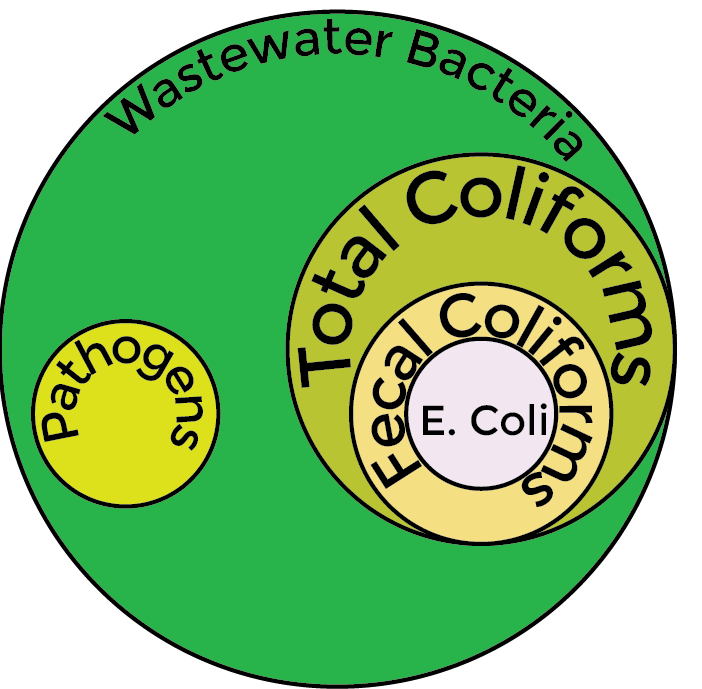
\includegraphics[width=4cm]{LaboratoryWastewaterBacteria}}
Wastewater Bacteria
\end{center}
	
	\item  In wastewater, fecal coliforms originate in the intestines of warm-blooded animals.  Aerobic bacteria including coliforms partake in the metabolization of the organic matter as part of the secondary treatment process
\item Fecal coliforms are seldom pathogenic under normal circumstances and are easily cultured, their presence indicates the potential presence of pathogens

The reason why these bacteria such as coliforms and enterococcus are used:
		\begin{enumerate}
			\item It is not practical to detect and quantify all pathogens associated with wastewater
			\item These bacteria originate from feces and indicate fecal contamination and thus serve as an indicator organisms for pathogens of wastewater origin
			\item They are also:
				\begin{itemize}
					\item abundant
					\item potentially less harmful, and
					\item easy to detect
				\end{itemize}
			\item \textit{E. coli} has been shown to be a better predictor of the potential for impacts to human health and therefore many newer wastewater discharge permits require \textit{E. Coli} testing in lieu of fecal coliform testing requirements.
		\end{enumerate}
		\end{enumerate}

\end{itemize}
 

\subsubsection{Bacteriological Testing Methods}\index{Bacteriological Testing Methods}
The methods for wastewater bacteriological tests include:  multiple-tube fermentation (MTF) technique, membrane filtration (MF) and quanti-tray testing.  When using the MTF and MF methods, it is not possible to exactly quantify the number of bacteria present, a statistical based - Most Probable Number (MPN) approach is utilized\\
\subsubsection{The Multiple-Tube Fermentation (MTF) technique}\index{The Multiple-Tube Fermentation (MTF) technique}
This involves adding three volumes – 10 ml, 1 ml and 0.1 ml of the sample, each to a set of five tubes containing Lauryl Tryptose broth and an inverted tube (Durham tube), followed by incubating the tubes at  for a specified time.  The Lauryl Tryptose broth produces color and/or turbidity change due to the growth of the target bacteria and the inverted tube collects the gas produced by the bacterial respiration.  At the end of the process, the number of tubes showing bacterial growth are counted for each volume of sample and using this information the concentrations of organisms in the original sample are established using Statistical Tables.  The test is conducted in three parts – presumptive, confirmative and completed.  A schematic of the MTF used for quantifying total coliforms and fecal coliforms is provided below.\\
\newpage
\thispagestyle{empty}
% \begin{landscape}
% \begin{center}
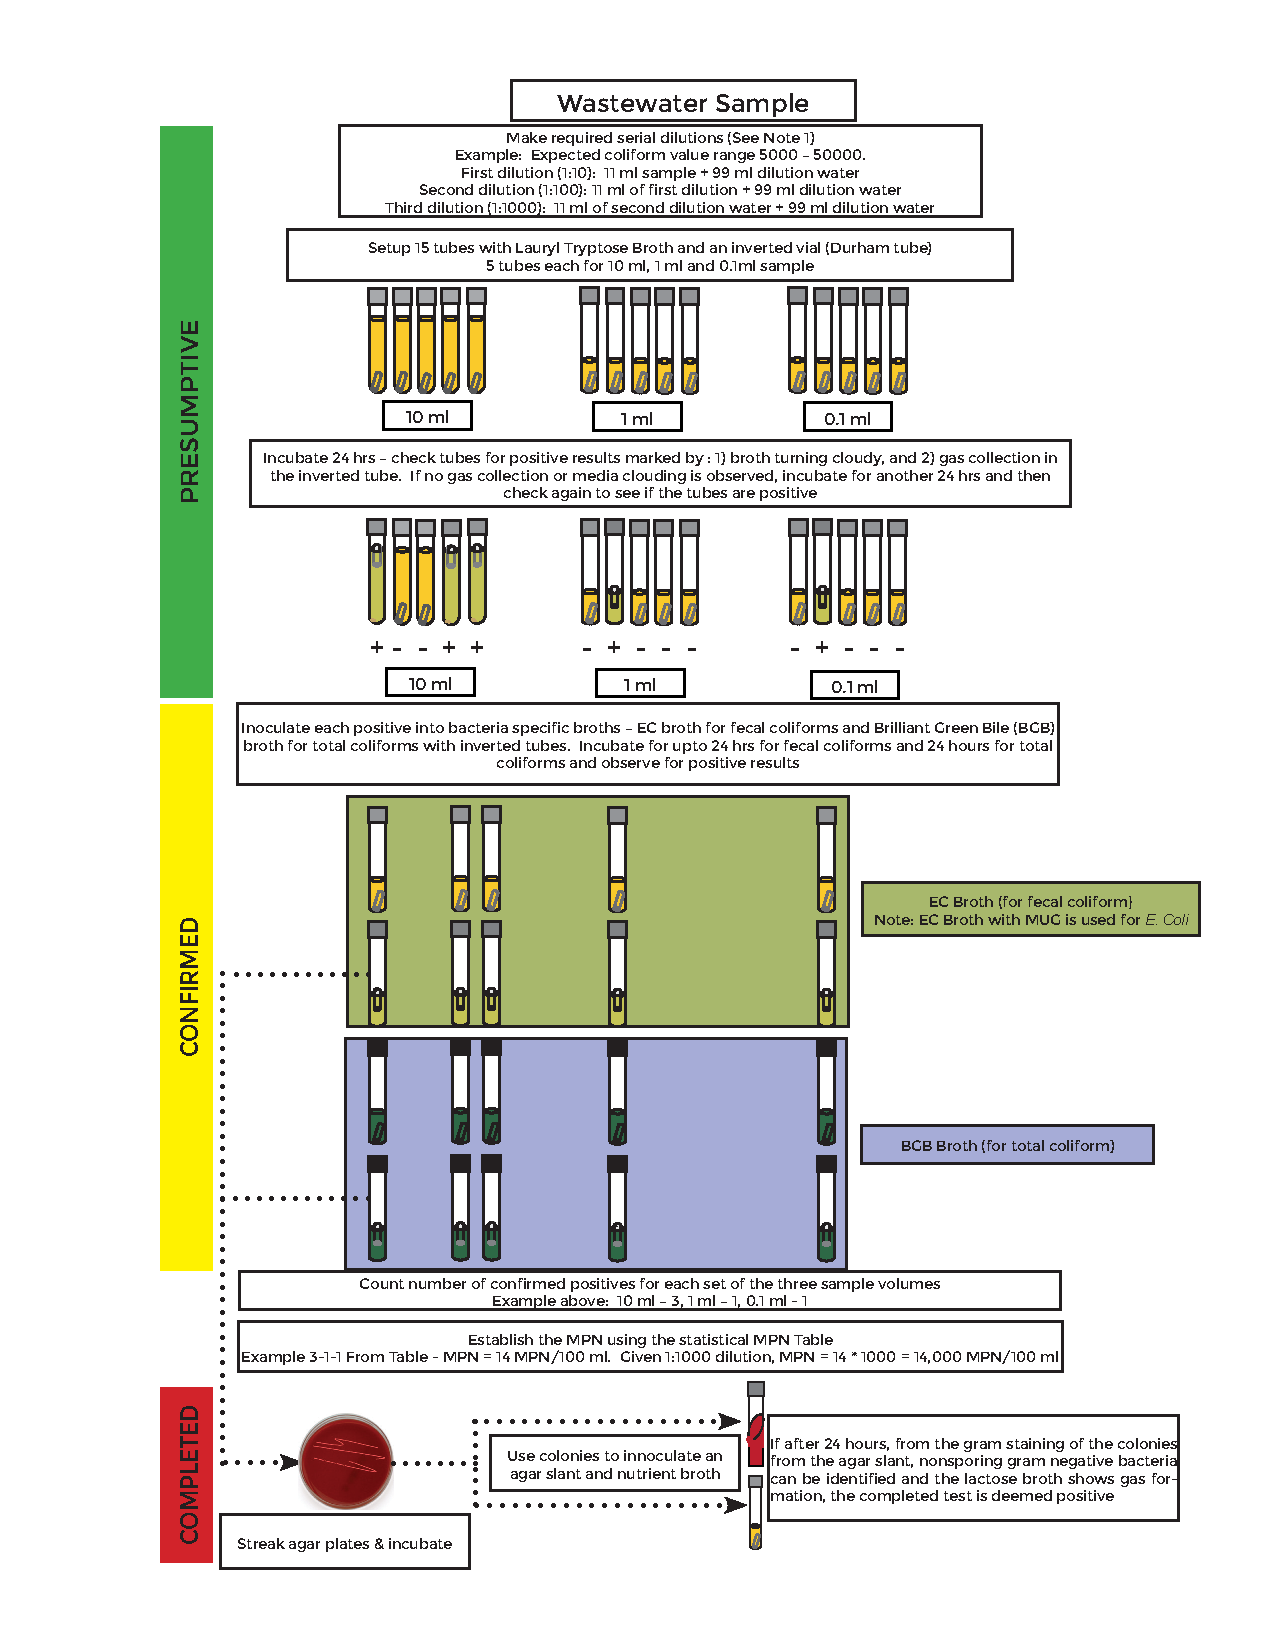
\includepdf[]{MTF.pdf}
%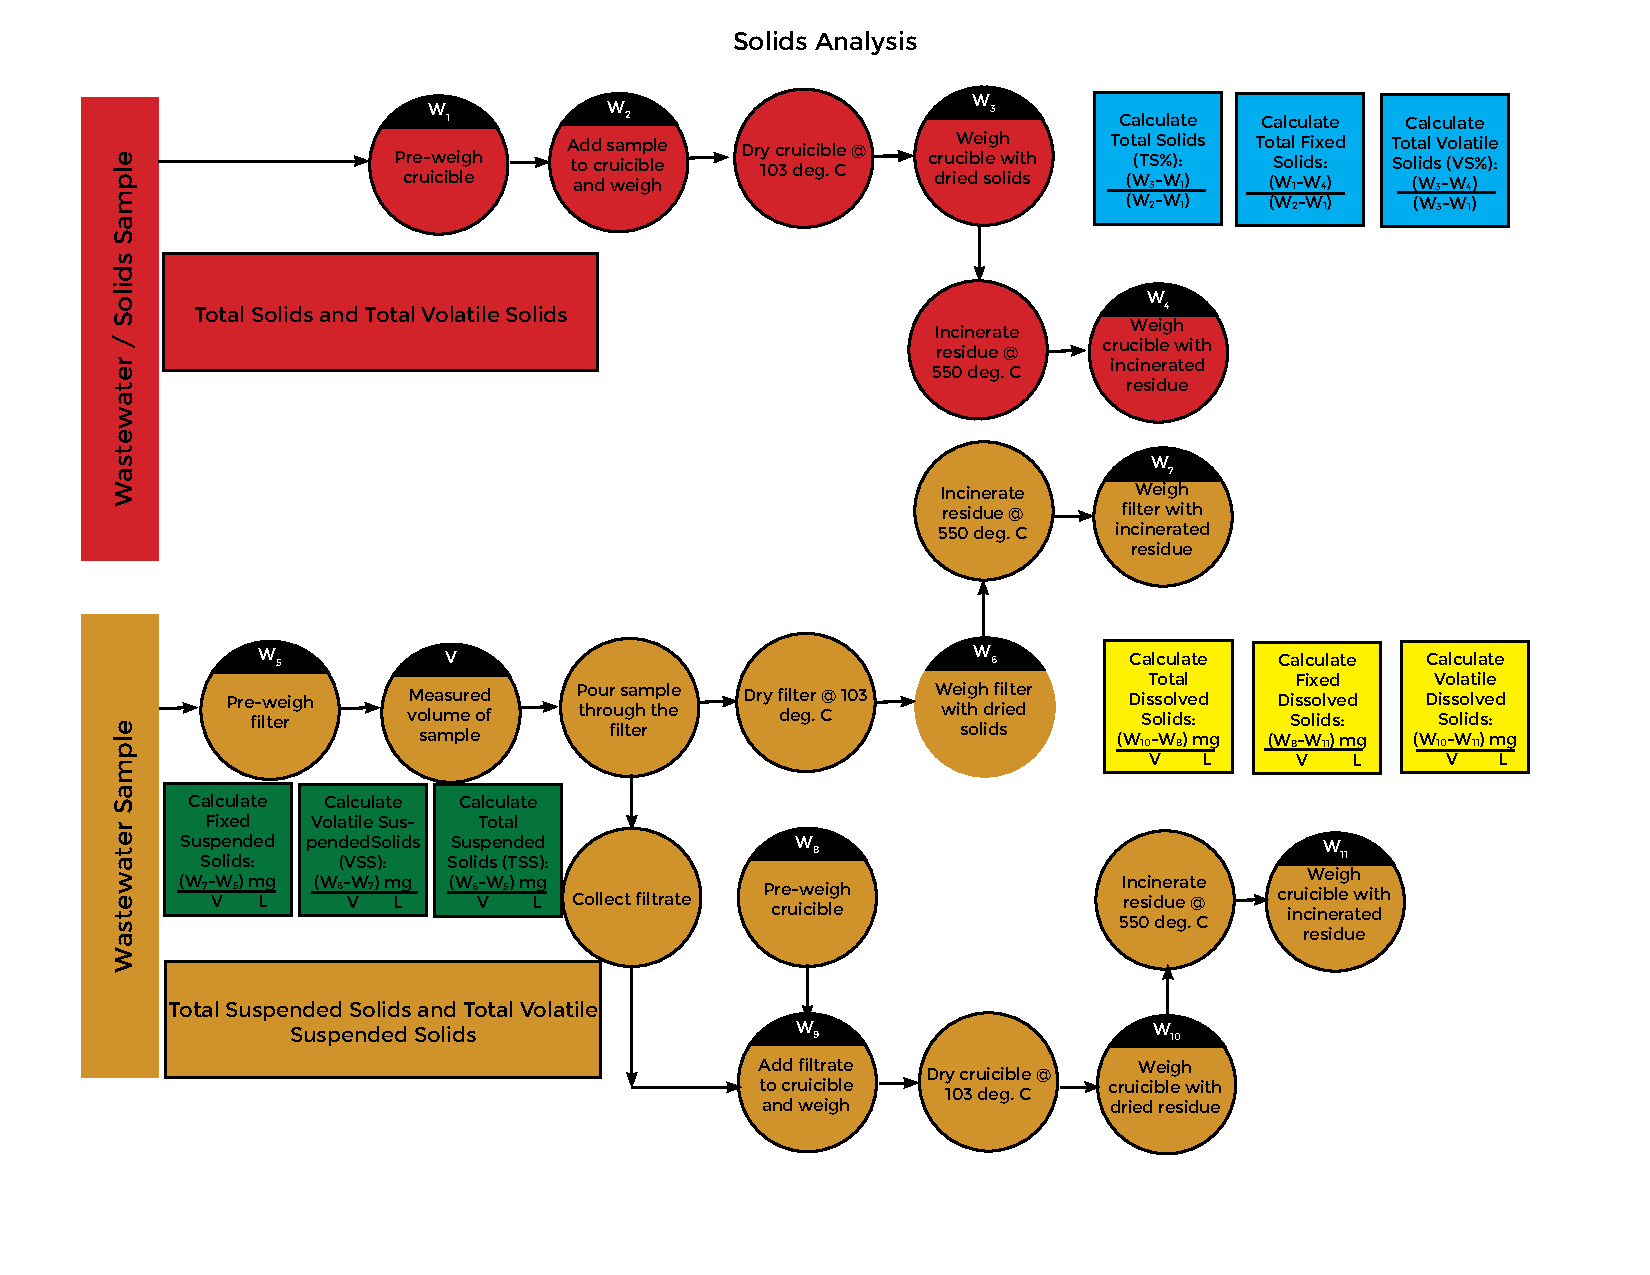
\includegraphics[scale=0.69]{LaboratorySolidsAnalysis4_01.pdf}
% \end{center}
% \end{landscape}
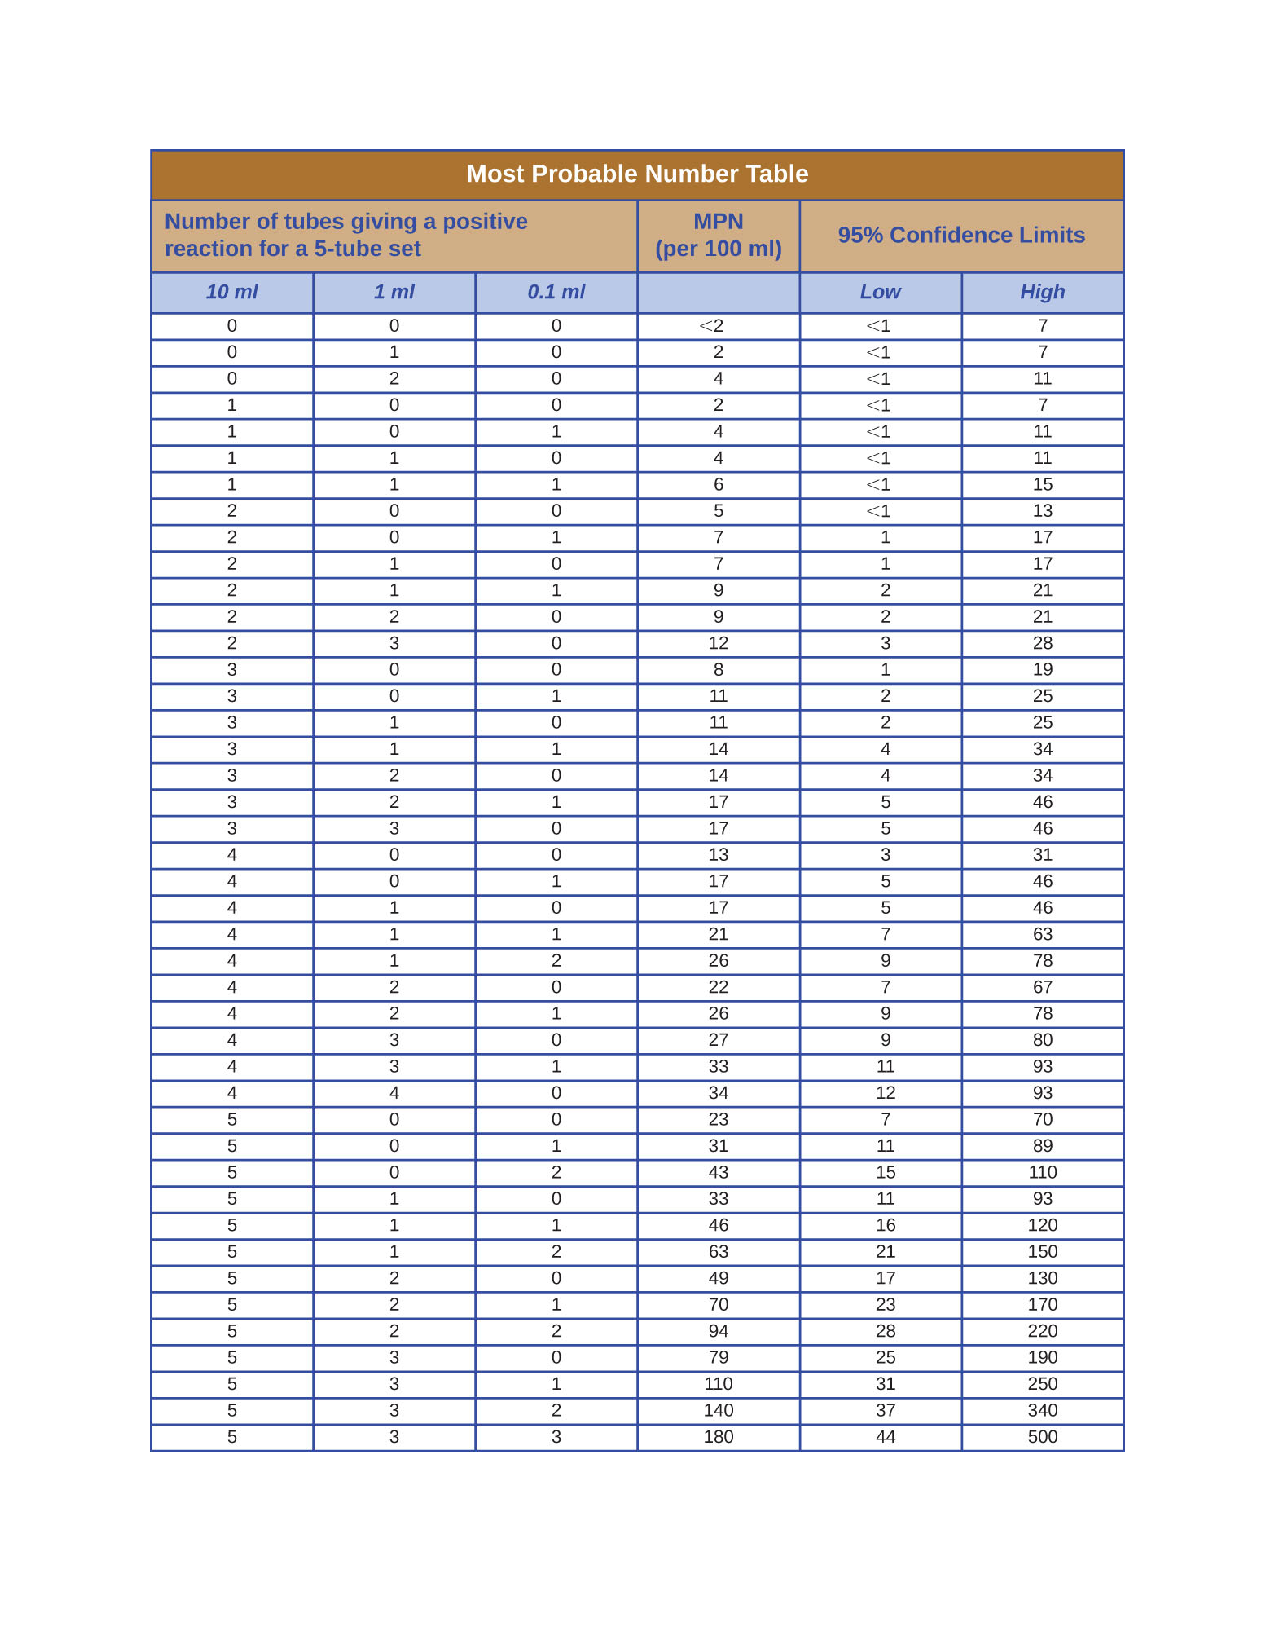
\includepdf[]{MTFTable.pdf}
\newpage
\subsubsection{The Membrane Filtration (MF) method}\index{The Membrane Filtration (MF) method}
This is a faster way to estimate bacterial populations in water.  In this method, an appropriate sample volume is passed through a membrane filter with a pore size small enough (0.45 micron) to retain the bacteria present. The filter is placed on an absorbent pad (in a petri dish) saturated with a culture medium that is selective for coliform growth. The petri dish containing the filter and pad is incubated, upside down, for 24 hours at the appropriate temperature. After incubation, the colonies that have grown are identified and counted using a low power microscope. A MUG medium is used for E- Coli.  If E. Coli is present, it will make the MUG fluorescent when viewed in UV light. 
\begin{center}
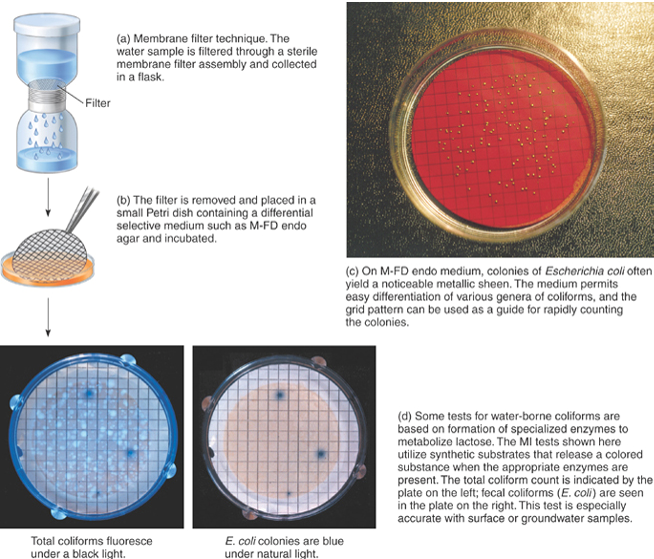
\includegraphics[scale=0.9]{LaboratoryMembraneFiltration}
\end{center}
\pagebreak

\subsubsection{Quanti-trays tests}\index{Quanti-trays tests}

This test used for the detection and quantification of specific microorganisms is being used increasingly mainly because it is a quicker test than the MTF.  Colilert and Enterolert are the quanti tray based tests for E. Coli and Enterococcus.  This method involve the use of specific enzymes and overcomes the drawbacks of the MTF which include false positives and negatives due to the more generic nature of the media used
\begin{center}
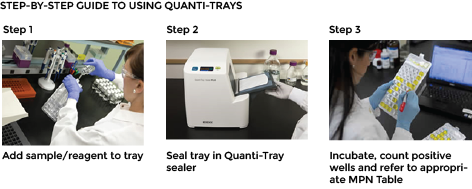
\includegraphics[scale=0.9]{LaboratoryQuantiTray}
\end{center}



